\documentclass[00-livre-main.tex]{subfiles}
\begin{document}

\chapter{The Equations of a Line in Space}

Let us now think about the nature of space. Okay, that sounded goofy. I don't mean contemplating planets and nebulae and the enormity of \emph{UY Scuti}. 
So far, all of our work has been in the plane, which is supposed to represent the ideal of a flat thing which is infinite in extent and ``two-dimensional.'' Our next theater for exploration is a model for the space in which we live. Rather than having two dimensions, it has three, so we can talk about motions which are not just forward and back, and right and left, but also up and down.

Fortunately, much of the hard work we have done understanding vectors in $\R^2$ carries over quickly. There are ready analogies for point, vector, and dot product, and though the geometry of these gets more interesting, the algebra really doesn't. That will eventually be our lifeline: as the spaces we consider get more exotic, the geometries will get more complicated (and eventually almost impossible to visualize), but the corresponding algebra will always have the same level of complexity. That is why the subject is called ``Linear Algebra'' rather than ``Linear Geometry.''

Drawing pictures becomes much more challenging. One option is to study drawing and painting for a few years until representing figures from space on a plane becomes more natural. In fact, there is a strong connection between linear algebra and some of the science behind perspective drawing, which mathematicians call \emph{projective geometry}. But as that is outside the plan of our current study, we will resort to images made with software.

Again, it will take some work to get there, but we are interested in the following question:

\begin{quotation}
\textbf{\large How can we clearly describe a single line in space with an equation?}
\end{quotation}


\section*{Points, Vectors, and the Dot Product in $\R^3$}

Just as we worked in the plane with points and vectors (both physicist's and mathematician's vectors) by using coordinates, we can do the same for the space around us. We have the same sort of muddled trichotomy to deal with, which should feel a little less mysterious by now. Anyway, a \emph{point} in space is supposed to be a location; a \emph{(physcist's) vector} is an arrow, having direction and magnitude; and a \emph{(mathematician's) vector} is an arrow whose tail is at a special, pre-selected point called the \emph{origin} and denoted by $O$.

There are many ways to attempt to set up coordinates in space, but experience has taught us that a good way mimics the set-up from the plane. There, in the plane, we used a pair of perpendicular lines through the origin as our backdrop, which we call \emph{coordinate axes}. In space, we have more room to deal with, so instead we use three planes as reference, and we try to make them as perpendicular as we can.

How do we arrange that? The key fact we need is that when distinct planes meet, they do so along a line. 
\begin{figure}[h]
\centering
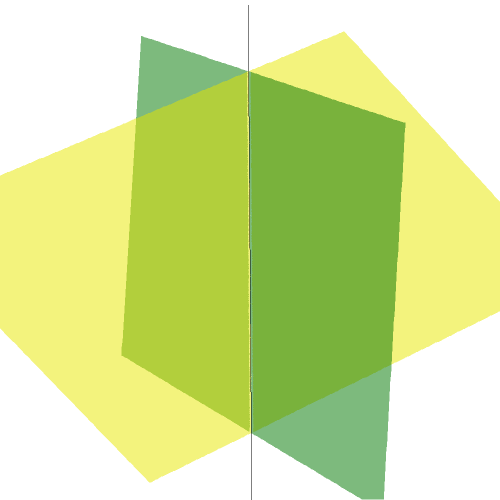
\includegraphics[width=0.3\textwidth]{images/two-planes-intersect.png}
\caption{Two planes intersect along a line.}
\label{fig:two-planes}
\end{figure}
Let's think through that a little. What does the picture look like near the intersection where two planes meet? A good way to understand it is to look ``across the intersection.'' To this end, turn the picture in front of you until the line of intersection is exactly the ``line of sight'' pointing directly away from your eye. If you do this correctly, the line should essentially vanish, by collapsing down to a single point in your vision. If you prefer, rather than imagining that you turn the picture, you can imagine moving around in space until you are in the line, and then looking in the correct direction. Either way, you should get the same image: the line of intersection collapses to a point, and the two planes under consideration collapse to lines in your vision, as you are looking at things ``edge on.''

This picture is now much simpler. We have turned the set-up of two planes which intersect along a line into a picture where two lines meet at a point. What we want is that these two lines should be perpendicular. In fact, they should mimic our usual coordinate axes picture for the plane.

So, now we are ready to set up our \emph{coordinate planes and axes} for space. First, choose a point $O$ to play the role of the origin. Then, through that point, choose three distinct planes $\p_1$, $\p_2$, and $\p_3$. Each pair of these planes meets along a line: call the intersection of plane $\p_i$ with plane $\p_j$ the line $\ell_{ij}$. So, for example, $\ell_{12}$ is the line along which plane $\p_1$ meets plane $\p_2$.

The important condition we want is this: If you look down the line $\ell_{ij}$, then the planes $\p_i$ and $p_j$ appear to be a pair of perpendicular lines. We require this to be true for each of the three lines $\ell_{ij}$ simultaneously.


\begin{figure}[h!]
\centering
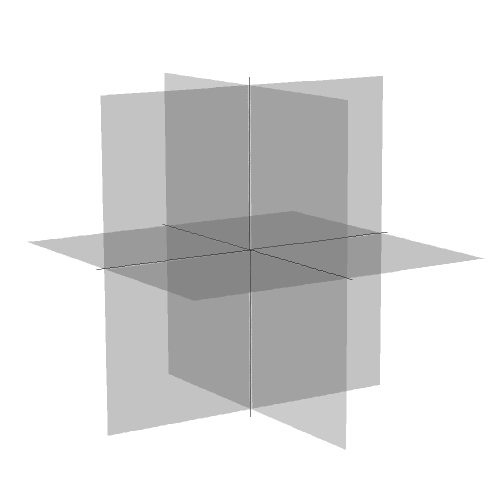
\includegraphics[width=.4\textwidth]{images/coord-planes.png}
\caption{The Coordinate Planes and Axes}
\label{fig:3d-coords}
\end{figure}

Now we are prepared to give some of these objects their traditional names. The planes $\p_1$, $\p_2$, and $\p_3$ are called the $yz$-plane, the $xz$-plane, and the $xy$-plane, respectively. The line $\ell_{12}$ is called the $z$-axis, the line $\ell_{23}$ is called the $x$ axis, and the line $\ell_{13}$ is called the $y$-axis.

Sometimes, instead of $x$, $y$, and $z$, we may use the variables $x_1$, $x_2$, and $x_3$. Then all of the names above change accordingly.

Just as in the plane, we can now introduce coordinates for points and vectors. We will just discuss how to do this for points, and you can see how to extend it to both interpretations of vectors in the same manner as before.

Given a point $P$ in space, draw a plane parallel to the $yz$-plane which passes through $P$. This plane will meet the $x$-axis in exactly one point. 
We treat the $x$-axis as a number line, so this point has associated to it a number $P_x$, which we call the \emph{$x$-coordinate of $P$}. 
Geometrically, the number $P_x$ represents the ``height'' of $P$ above the $yz$-plane. 
The words height and above are used in a relative sense, here.

Similarly, we can draw a plane parallel to the $xz$-plane which passes through $P$. This plane will intersect the number line of the $y$-axis, and we call the corresponding number $P_y$ the \emph{$y$-coordinate of $P$}. 
Finally, we can draw a plane parallel to the $xy$-plane through $P$, which will intersect the $z$-axis in a point, whose corresponding number $P_z$ is called the \emph{$z$-coordinate of $P$}. 
We then take these three numbers and bundle them together and represent the point $P$ by the ordered triple $P = (P_x, P_y, P_z)$.
Just as before, we will distinguish between points and vectors in our notation, and write vectors as vertical stacks of numbers. Here, such a stack has three parts. Motivated by our work in the plane, we make the following definition.

\begin{definition} 
A $3$-vector is a vertical stack of three real numbers, like so:
\[
v = \begin{pmatrix} v_x\\ v_y \\ v_z\end{pmatrix}.
\]
The collection of all such $3$-vectors is called \emph{$3$-space}, and written with this notation: $\R^3$.
\end{definition}

The notation $\R^3$ is often read as ``arr-three,'' and many people use that language in place of ``three-space.'' Also, most of the time we will just say ``vector'' when the context is clear. But it can be helpful to have the extra bit of information in situations where vectors of different sizes are involved.

The algebra of $3$-vectors is handled in exactly the same way as the algebra of $2$-vectors, except that there is another coordinate to track. All of the geometric connections between points, mathematician's vectors, and physicist's vectors work just as before, but there is ``more space'' to work with. Most people find visualization in three-space to be much harder than in the plane. This is completely normal, and you should expect to get used to this only if you work at it.

\begin{definition}[Algebra in $\R^3$]
Suppose that $u$ and $v$ are $3$-vectors, and that $\lambda$ and $\mu$ are scalars (real numbers). Then the \emph{linear combination of $u$ and $v$ with weights $\lambda$ and $\mu$} is defined coordinate-by-coordinate:
\[
\lambda u + \mu v = \lambda \begin{pmatrix} u_x \\ u_y \\ u_z \end{pmatrix} +
\mu \begin{pmatrix} v_x \\ v_y \\ v_z \end{pmatrix} =  
\begin{pmatrix} \lambda u_x + \mu v_x \\ \lambda  u_y + \mu v_y \\ \lambda u_z + \mu v_z \end{pmatrix} 
\]
\end{definition}

It is, of course, possible to form linear combinations of larger collections of vectors, using the corresponding number of weights. You should also notice that addition of $3$-vectors and scalar multiplication for $3$-vectors are special cases of linear combination. (How would you do this? Check this statement!) The statements of Theorem \ref{thm:vect-add} and Theorem \ref{thm:scalar-mult} carry over unchanged to our new setting. The algebra of vectors behaves just as sensibly in $\R^3$ as in $\R^2$, even if the pictures are more challenging.

The geometry of $\R^3$ can be handled similarly, too, with dot products, norms, and angles. 

\begin{definition}[Dot Product, norm, and angles in $\R^3$]
Let $u$ and $v$ be $3$-vectors. The \emph{dot product} of $u$ and $v$ is the real number
\[
u \cdot v = \begin{pmatrix} u_x \\ u_y \\ u_z \end{pmatrix} \cdot \begin{pmatrix} v_x \\ v_y \\ v_z \end{pmatrix} = u_x v_x + u_y v_y + u_z v_z,
\]
the \emph{norm} of $u$ is the non-negative real number
\[
\norm{u} = \sqrt{u\cdot u\ } = \sqrt{ u_x^2 + u_y^2 + u_z^2\ }, 
\]
and the angle between $u$ and $v$ is defined to be 
\[
\theta = \arccos\left( \dfrac{u\cdot v}{\norm{u}\norm{v}} \right). 
\]
We say two vectors are \emph{orthogonal} when their dot product is $0$. A vector is called a \emph{unit vector} when its norm is equal to $1$.
\end{definition}

Again, these behave just as well in $\R^3$ as in $\R^2$. It is possible to ``normalize'' a non-zero vector $u$ to produce a unit vector $\norm{u}^{-1} u$, and the statement of Theorem \ref{thm:dot-prod-props} works in $\R^3$.


\section*{Parametric lines}

lines in R3 parametrically: through the origin, not

\section*{Describing Planes in $3$-space}

\textbf{Outline}
\begin{compactitem}
\item planes in R3 parametrically: through the origin, not
\item normal vector to a plane
\item the shape of things normal to a line
\item the equation of a plane: by elimination, by dot product
\item families of parallel planes
\item sketching from an equation
\item big theorem with duality for planes
\end{compactitem}

\section*{Lines in $\mathbb{R}^3$ as Solutions to Systems of Equations}

LINES in R3 as intersection of two planes, cases of concern

parametric to equations and back

\end{document}